\section{Exploratory Data Analysis}
\label{sec:eda}

We ran the analysis on the training split only and organised it around six feature groups, each chosen to answer one question about the task (\cref{tab:eda-groups}). We left out lexical-richness measures such as TTR, MTLD and HD-D on purpose: on three-word phrases they are undefined, or they jump around with a single word. The seven figures of the analysis are collected, without captions, in the separate EDA PDF. Two of them appear here.

\begin{table}[t]
\centering
\small
\begin{tabular}{@{}p{0.25\columnwidth}p{0.67\columnwidth}@{}}
\toprule
Group & Question \\
\midrule
Length & Does the longer phrase predict the direction? \\
Readability & Do word and syllable lengths differ by relation? \\
Lexical & Do overlap and containment separate direction, equivalence and negatives? \\
Semantic & Does embedding similarity separate the relations, and can it see direction? \\
Linguistic & Do heads, POS patterns, adjectives and prepositions vary by relation? \\
Task cues & Are quantifiers, negation, numerals and named entities frequent enough to matter? \\
\bottomrule
\end{tabular}
\caption{The six EDA feature groups and the question each answers.}
\label{tab:eda-groups}
\end{table}

\paragraph{Length.}
\textit{Observation.} The premise is the longer phrase in 78\% of \FW{} instances and the hypothesis in 78\% of \BW{} instances. \EQ{} splits almost evenly (36\% premise longer, 29\% equal, 36\% hypothesis longer), and about half of the \NO{} instances (49\%) have the same length on both sides (\cref{fig:length}). \textit{Interpretation.} Direction leaks through form. The entailing phrase is usually the more specific one, and specificity in this data is mostly added words (``in Russia'' against ``in Russian city of Kazan''), so a model can learn direction without touching meaning. \textit{Implication.} Length goes into the cue baseline. Every model also gets scored separately on the instances where length points the wrong way or nowhere (\cref{sec:error}), because those are the ones that tell us whether anything beyond the shortcut was learned.

\begin{figure}[t]
\centering
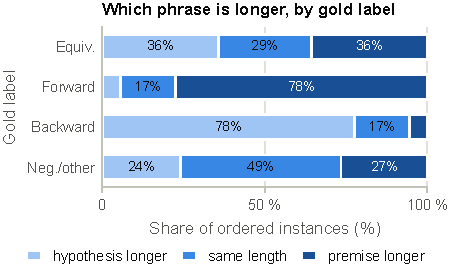
\includegraphics[width=\columnwidth]{figures/eda-length-cue}
\caption{Which phrase is longer, by gold label (train).}
\label{fig:length}
\end{figure}

\paragraph{Lexical overlap and containment.}
\textit{Observation.} Mean word-set Jaccard overlap is 0.41 for directional pairs, against 0.24 for \EQ{} and 0.27 for \NO{}. Containment is one-sided: every hypothesis word occurs in the premise in 45\% of \FW{} instances and only 2\% of \BW{} instances, and the mirror holds for the other direction. The last word is shared in 58\% of directional instances (\cref{fig:lexical}). \textit{Interpretation.} A directional pair is typically one phrase with words added or removed around a head that stays put. Equivalences look different. They are paraphrases, often with little literal overlap: ``Woman and dog'' and ``an adult female accompanied by a dog'' share one word. \textit{Implication.} Containment in both orientations is a strong direction cue when it fires, but it fires on fewer than half of the directional pairs. Overlap tells a model that two phrases are related; it does not tell it that they are equivalent.

\begin{figure*}[t]
\centering
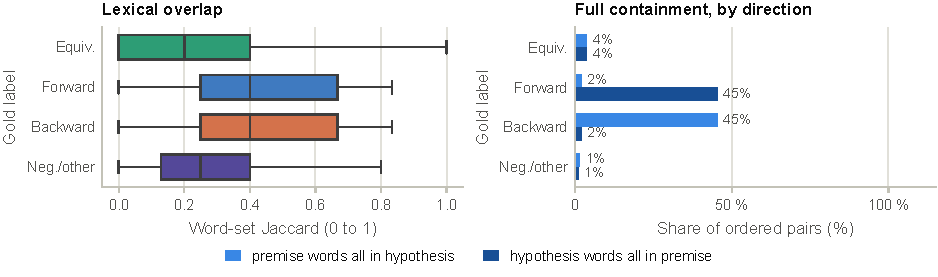
\includegraphics[width=\textwidth]{figures/eda-lexical-containment}
\caption{Word overlap (left) and full containment in each direction (right), by gold label (train).}
\label{fig:lexical}
\end{figure*}

\paragraph{Semantic similarity.}
\textit{Observation.} Cosine similarity of MiniLM sentence embeddings \citep{reimers-gurevych-2019-sentence} has a median of 0.76 for \EQ{}, 0.77 for both directions and 0.64 for \NO{}. 52\% of directional and 50\% of \EQ{} instances sit at or above the \EQ{} median, against 27\% of negatives. Cosine is symmetric, so a pair and its reversal get exactly the same value. \textit{Interpretation.} Similarity separates negatives from related pairs, moderately, and does nothing for the line between \EQ{} and entailment. It carries no information about direction, by construction. \textit{Implication.} We kept cosine out of the cue set. A symmetric representation cannot recover direction, and the equivalence boundary needs something that reads the ordered pair, which is what we expected the encoder to supply.

\paragraph{Linguistic and task-specific cues.}
\textit{Observation.} The two heads share a lemma in 52\% of directional instances against 30\% of \EQ{}. The part-of-speech pattern is identical on both sides in 31\% of \NO{} instances and only 7\% of directional ones. The premise of a \FW{} pair carries 0.33 more adjectives, on average, than its hypothesis. Numerals occur in 18\% of directional instances and named entities in 47\%; quantifiers (3\%) and negation (under 1\%) are rare. \textit{Interpretation.} A negative is often one substituted word inside an unchanged frame (``Two young children'' against ``Two small children'' is labelled \NO{}), and adjectives are the material that narrows a phrase. \textit{Implication.} Comparing heads and modifiers should matter more than any global similarity. Quantifiers and negation are too rare to train on, so we keep them as error-analysis slices instead.

\paragraph{Readability.}
\textit{Observation.} Syllables per word run from 1.53 to 1.60 across labels, characters per word from 4.5 to 4.9, and median Flesch reading ease from 77.9 to 82.4. \textit{Interpretation.} The phrases are uniformly short caption and headline language. Flesch assumes sentences, and on fragments it only tracks syllable density. \textit{Implication.} Readability does not separate the labels and stays out of the feature set. It stays in the report so that nobody has to rerun the check.
